% --------------------------------------------------------------
% This is all preamble stuff that you don't have to worry about.
% Head down to where it says "Start here"
% --------------------------------------------------------------
 
\documentclass[12pt]{article}
 
\usepackage[margin=1in]{geometry} 
\usepackage{amsmath,amsthm,amssymb,scrextend}
\usepackage{fancyhdr}
\usepackage{enumitem}
\usepackage{amsmath}
\usepackage{amssymb}
\usepackage{textcomp}
\usepackage{fancybox}
\usepackage{tikz}
\usepackage{tasks}
\pagestyle{fancy}
\usepackage[makeroom]{cancel}
\usepackage{graphicx}
\usepackage{caption}
\usepackage{mwe}
\usepackage{tikz}
\usetikzlibrary{positioning}

\newcommand{\N}{\mathbb{N}}
\newcommand{\Z}{\mathbb{Z}}
\newcommand{\I}{\mathbb{I}}
\newcommand{\R}{\mathbb{R}}
\newcommand{\Q}{\mathbb{Q}}
\renewcommand{\qed}{\hfill$\blacksquare$}
\let\newproof\proof
\renewenvironment{proof}{\begin{addmargin}[1em]{0em}\begin{newproof}}{\end{newproof}\end{addmargin}\qed}
% \newcommand{\expl}[1]{\text{\hfill[#1]}$}
 
\newenvironment{theorem}[2][Theorem]{\begin{trivlist}
\item[\hskip \labelsep {\bfseries #1}\hskip \labelsep {\bfseries #2.}]}{\end{trivlist}}
\newenvironment{lemma}[2][Lemma]{\begin{trivlist}
\item[\hskip \labelsep {\bfseries #1}\hskip \labelsep {\bfseries #2.}]}{\end{trivlist}}
\newenvironment{problem}[2][Problem]{\begin{trivlist}
\item[\hskip \labelsep {\bfseries #1}\hskip \labelsep {\bfseries #2.}]}{\end{trivlist}}
\newenvironment{exercise}[2][Exercise]{\begin{trivlist}
\item[\hskip \labelsep {\bfseries #1}\hskip \labelsep {\bfseries #2.}]}{\end{trivlist}}
\newenvironment{reflection}[2][Reflection]{\begin{trivlist}
\item[\hskip \labelsep {\bfseries #1}\hskip \labelsep {\bfseries #2.}]}{\end{trivlist}}
\newenvironment{proposition}[2][Proposition]{\begin{trivlist}
\item[\hskip \labelsep {\bfseries #1}\hskip \labelsep {\bfseries #2.}]}{\end{trivlist}}
\newenvironment{corollary}[2][Corollary]{\begin{trivlist}
\item[\hskip \labelsep {\bfseries #1}\hskip \labelsep {\bfseries #2.}]}{\end{trivlist}}
 
\setlength{\parindent}{0pt}
\begin{document}
 \settasks{
	counter-format=(tsk[r]),
	label-width=4ex
}
% --------------------------------------------------------------
%                         Start here
% --------------------------------------------------------------

\lhead{Math 632}
\chead{Practice Exam}
\rhead{Meenmo Kang}

\begin{enumerate}
\item 
    \begin{enumerate}

    \item     $$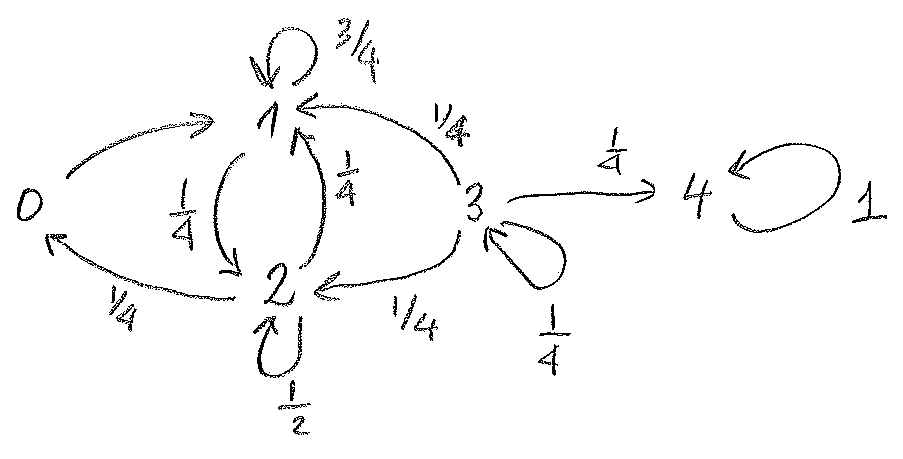
\includegraphics[height=5cm, width=10cm]{PE_1.PNG}$$
    \begin{itemize}
        \item Closed irreducible recurrent sets: $\{0,1,2\}, \{4\}$
        \item Transient: $\{3\}$
    \end{itemize}
    
    \item 
    \begin{align}
        P_3(T_4<\infty) &= \sum\limits_{k=1}^\infty P_3(T_4=k)
    =\sum\limits_{k=1}^\infty P_3(x_1 = ... = x_{k-1} = 3,\;x_k=4) \nonumber \\
    &=\sum\limits_{k=1}^\infty\left(\frac{1}{4}\right)^k = \frac{1}{3} \nonumber
    \end{align}
    
    \item 
    \begin{itemize}
        \item $\lim\limits_{n\to\infty}p^n(2,1) = \pi(1) = \frac{8}{13}$
        \item $\lim\limits_{n\to\infty}p^n(1,2) = \pi(2) = \frac{4}{13}$
        \item $E_0[T_0] = 1/\pi(0)$
    \end{itemize}
    
    \item $\lim\limits_{n\to\infty} p^n(3,1) = (1-1/3)\cdot \pi(1) = \frac{2}{3}\cdot\pi(1)$
    \end{enumerate}
    
    
    
    \item 
    \begin{itemize}
        \item The distribution of patrol's cycle
        $$g(z) = \frac{P(t_i>z)}{E[t_i]}=1/2\qquad \text{   if $0\le z \le 2$}$$
        
        \begin{align}
            P(T>R+2) &= P(R<T-2) = P(2\le T\le 4,\; 0<R<T-2)\nonumber \\
            &=\int_2^4\int_0^{t-2} \frac{1}{4}\frac{1}{2}drdt = \int_2^4 \frac{1}{8}(t-2) dt \nonumber \\
            &=\frac{1}{8}\left[\frac{t^2}{2}-2t\right]_2^4 = \frac{1}{4}\nonumber   
        \end{align}
    \end{itemize}
    
    \newpage
    \item $$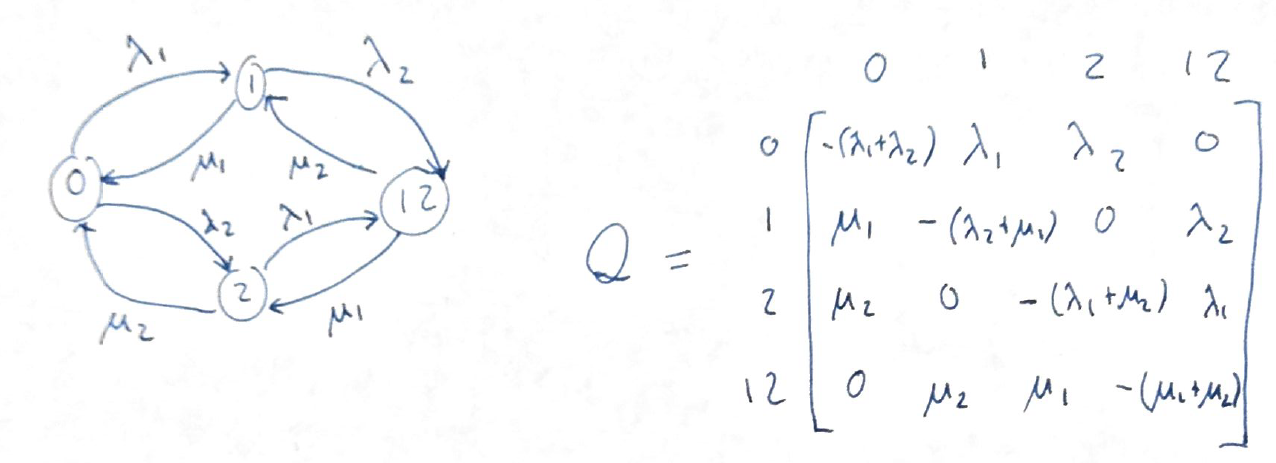
\includegraphics[height=5cm, width=11cm]{PE_2.PNG}$$
    
    $$
        \begin{cases}
        \pi(0)\lambda_2 = \pi(2)\mu_2\\
        \pi(0)\lambda_1 = \pi(1)\mu_1\\
        \pi(12)\mu_1 = \pi(2)\lambda_1\\
        \pi(12)\mu_2 = \pi(1)\lambda_2\\
        \end{cases}
        \begin{cases}
        \pi(2) = \frac{\lambda_2}{\mu_2}\pi(0)\\
        \pi(1) = \frac{\lambda_2}{\mu_1}\pi(0)\\
        \pi(12) = \frac{\lambda_1}{\mu_1}\pi(2)=\frac{\lambda_1\lambda_2}{\mu_1\mu_2}\pi(0)\\
        \pi(12) = \frac{\lambda_2}{\mu_2}\pi(1)=\frac{\lambda_1\lambda_2}{\mu_1\mu_2}\pi(0)
        \end{cases}
    $$
    
    \begin{align}
        \pi(0)+\pi(1)+\pi(2)+\pi(12) &= \pi(0)\left(1 + \frac{\lambda_2}{\mu_1} +  \frac{\lambda_2}{\mu_2} + \frac{\lambda_1\lambda_2}{\mu_1\mu_2}\right) = 1 \nonumber \\
        \pi(0) &= \frac{1}{\left(1 + \frac{\lambda_2}{\mu_1} +  \frac{\lambda_2}{\mu_2} + \frac{\lambda_1\lambda_2}{\mu_1\mu_2}\right)}
        =\frac{1}{\left(1+\frac{\lambda_1}{\mu_1}\right) \left(1+\frac{\lambda_2}{\mu_2}\right)}\nonumber\\
        \pi(12)&=\frac{\lambda_1\lambda_2}{\mu_1\mu_2}\cdot \frac{1}{\left(1+\frac{\lambda_1}{\mu_1}\right) \left(1+\frac{\lambda_2}{\mu_2}\right)}=\frac{\lambda_1\lambda_2}{(\mu_1+\lambda_1)(\mu_2+\lambda_2)} \nonumber
    \end{align}
    
    \item \begin{align}
        P(\text{I leave first}) &= 
        \sum\limits_{k=0}^\infty P(\text{$k$ customers present, $T_0<\min\limits_{1\le i\le k}T_i$)}\nonumber \\
        &=\sum\limits_{k=0}^\infty \frac{-e^{-\frac{\lambda}{\mu}}\left(\frac{\lambda}{\mu}\right)^k}{k!}\cdot \frac{1}{k+1}= e^{-1/\mu}\frac{\mu}{\lambda} \sum\limits_{k=0}^\infty \frac{\left(\frac{\lambda}{\mu}\right)^{k+1}}{(k+1)!}  \nonumber \\
        &=e^{-\frac{\lambda}{\mu}} \frac{\mu}{\lambda} \left(e^{\lambda/\mu}-1\right) = \frac{\mu}{\lambda}\left(1-e^{-\lambda/\mu}\right) \nonumber
    \end{align}
\end{enumerate}

\end{document}
